\documentclass[11pt]{article}
\usepackage[margin=0.9in]{geometry}
\usepackage{amsmath,amssymb,amsthm,booktabs,longtable,array,hyperref}
\usepackage{pgfplots}
\usepgfplotslibrary{groupplots}
\pgfplotsset{compat=1.18}
\hypersetup{colorlinks=true,linkcolor=blue,urlcolor=blue}
\setlength{\emergencystretch}{3em}
\newtheorem{theorem}{Theorem}
\newtheorem{lemma}{Lemma}
\newtheorem{corollary}{Corollary}
\newcommand{\diag}{\operatorname{diag}}
\newcommand{\Cov}{\operatorname{Cov}}
\newcommand{\Var}{\operatorname{Var}}
\newcommand{\Mp}{M}
\title{A counterexample to the four state Mpemba triplet conjecture}
\author{Research report and reproducible mathematical certificate}
\date{11 October 2026}
\begin{document}
\maketitle
\begin{abstract}
The four-state implication specified in the assignment is false. An explicit reversible generator with strictly positive rates and four distinct energies fails the necessary-condition test of Avitan, Factor and Gelbwaser-Klimovsky on every original-rate triplet, but has an ordinary asymptotic cooling Mpemba effect between two finite positive initial temperatures. The bath inverse temperature is one; the initial inverse temperatures are $1/1000$ and $1/100$. Rational interval arithmetic certifies the thermal-overlap inequality. The example has a simple slow mode and strict margins, hence belongs to an open family of counterexamples. We connect the triplet inequalities to established stochastic monotonicity, obtaining corrected sufficient conditions for absence. The supporting order argument is presented as an application of existing theory, with explicit comparison to Ohga, Hayakawa and Ito. Overlap plots and a certified finite-time distance crossing show the physical effect, whose amplitude advantage is about 0.1102\%.
\end{abstract}

\section{Outcome}
The proposed triplet test can miss a genuine four-state relaxation reversal. In the example, the hotter preparation begins farther from equilibrium, yet later becomes slightly closer. The reversal is mathematically rigorous and physically small. Every input rate and bath weight is rational. The energies are logarithms of those weights. A cubic with integer coefficients specifies the slow eigenvalue, and cofactor polynomials specify its left eigenvector exactly. Thermal probabilities at the two selected temperatures are algebraic numbers bounded by rational numbers whose correctness is checked by integer powers.

A companion example has an exactly rational slow eigenvalue and left eigenvector. It gives a second, simpler spectral certificate, at the expense of two less compact rates. Both examples are strictly inside the required positive-rate and simple-slow-mode domain. No assertion about a strong Mpemba effect is needed: the two displayed slow-mode overlaps are nonzero.

\section{Problem and literature status}
The target is the inference that failure of Eq.~(3) on every energy-ordered triplet of a four-state reversible thermalizing generator precludes the Mpemba effect. The triplets retain the original off-diagonal rates. This is the conjecture in \href{https://arxiv.org/html/2603.04567v1}{Avitan, Factor and Gelbwaser-Klimovsky, arXiv:2603.04567v1}, submitted 4 March 2026. Its main text and supporting information, particularly S2--S14, were checked on 11 October 2026. The version history listed only v1. Its finite-temperature claim is numerical; the analytic theorem assumes zero bath temperature and stronger triplet inequalities.

The later \href{https://arxiv.org/html/2609.09988v1}{Gelbwaser-Klimovsky, arXiv:2609.09988v1}, submitted 9 September 2026, repeats the inference without providing a general proof. Its examples without an exact three-state mechanism concern a different, stronger predicate. Searches by title, identifier, conjecture, correction and counterexample located no other primary-source resolution. This establishes the scope of the literature check; it does not exclude unindexed or unpublished work. The target was not changed. Publication priority or exhaustive novelty is not claimed.

For supporting no-Mpemba results we additionally checked \href{https://arxiv.org/html/2410.06623v2}{Ohga, Hayakawa and Ito, arXiv:2410.06623v2}, version-history date 19 October 2024, including Result 2 and SI B--D, on 11 October 2026. Their theorem is a prior application of monotone coupling to absence of mean-energy crossings. Section~\ref{sec:priororder} compares the assumptions and observables precisely. We do not claim a new general monotonicity principle.

For definitions we use \href{https://pmc.ncbi.nlm.nih.gov/articles/PMC5441807/}{Lu and Raz, PNAS 114, 5083--5088 (2017)}, and distinguish the strong effect of \href{https://arxiv.org/abs/1711.05829}{Klich et al., Phys. Rev. X 9, 021060 (2019)}. The asymptotic conclusion is supplemented below by certified finite-time crossing brackets.

\subsection{Model and reductions}
With column probabilities, $\dot p=Mp$, $M_{ij}=a_{ij}$ for $i\ne j$, and $M_{jj}=-\sum_{i\ne j}a_{ij}$. The rate $a_{ij}$ goes from $j$ to $i$. Write
\[
q_i=e^{-\beta_b E_i},\qquad Q=\sum_iq_i,\qquad \pi_b=q/Q.
\]
Detailed balance is $M_{ij}q_j=M_{ji}q_i$. An energy shift sets $E_1=0$; measuring energies in bath units sets $\beta_b=1$. A common positive multiplier of $M$ changes only the time unit. We use $a_{12}=1$. We neither assume equally spaced energies nor normalize the total energy span. These would impose additional restrictions.

If $D=\diag(\pi_b)$, detailed balance makes $S=D^{-1/2}MD^{1/2}$ symmetric: $MD=DM^\top$. Hence the spectrum is real and the generator is diagonalizable. Its Dirichlet form is
\[
-f^\top D M^\top f=\sum_{i<j}c_{ij}(f_i-f_j)^2,\qquad c_{ij}=M_{ij}\pi_{bj}=c_{ji}.
\]
In the positive-rate domain the stationary eigenvalue is simple. The slowest nonzero eigenvalue is additionally assumed simple and is certified below.

\subsection{Exact predicate and its negation}
For $i<j<k$, put $A=a_{ik}$, $B=a_{jk}$, $C=a_{ij}$, $t=q_j/q_i$, $u=q_k/q_j$. The source's $(-,0,+)$ correspond to $(i,j,k)$. Its exact test is
\begin{align*}
\kappa&=\frac{A+B}{C(1+t)},&G&=At-B,\\
F&=A(1+tu/2)-B(1+u/2)-C(1-t),\\
P_{ijk}&=(\kappa\geq1\ \land\ F>0)\ \lor\ (\kappa\leq1\ \land\ G>0).
\end{align*}
Both strict comparisons and both inclusive branch comparisons match Eq.~(3) and S9. The assignment's transcription is correct.

\begin{lemma}[The branch logic reduces to a convex cone]
For positive $C$ and $0<t<1$, $\neg P_{ijk}$ is equivalent to $F\leq0$ and $G\leq0$.
\end{lemma}
\begin{proof}
Let $H=A+B-C(1+t)$, $d=(1-t)/(1+t)>0$, and $h=2/(1+t)+u/2>0$. Direct expansion gives $F=hG+dH$. If $H>0$, failure is $F\leq0$, which forces $G<0$. If $H<0$, failure is $G\leq0$, which forces $F<0$. At $H=0$ both branches apply, but $F=hG$, so their strict tests agree. These cases prove both directions.
\end{proof}
For fixed energies the eight linear inequalities define one closed polyhedral cone. The admissible rates are its intersection with the strictly positive orthant. This conclusion does not discard the original branch logic; it proves an equivalent formulation including $\kappa=1$.

The supporting-information fast-vector formulas divide by $-uG$. We do not use that division. When $G=0$, direct triplet diagonalization gives nonzero eigenvalues $-A(1+t+tu)$ and $-[C(1+t)+Atu]$. If also $H=0$, they coincide. The predicate remains well-defined whenever $C>0$. Isolated triplet generators require their diagonals to be recomputed, not inherited as principal submatrices.

\subsection{What the cooling witness proves}
Choose $Mv_2=\lambda_2v_2$, $w_2^\top M=\lambda_2w_2^\top$ and $w_2^\top v_2=1$. Since $\lambda_2\ne0$, $w_2^\top\pi_b=0$. Thus
\[
b_2(\beta)=w_2^\top[\pi(\beta)-\pi_b]=w_2^\top\pi(\beta).
\]
All initial temperatures here are finite and positive. Cooling has $0<\beta_h<\beta_c<\beta_b$, with anomalous ordering $|b_2(\beta_h)|<|b_2(\beta_c)|$. Heating instead has $\beta_b<\beta_h<\beta_c$ and requires $|b_2(\beta_c)|<|b_2(\beta_h)|$.

With a simple slow mode,
\[
p(t;\beta)-\pi_b=e^{\lambda_2t}b_2(\beta)v_2+O(e^{\lambda_3t}).
\]
Consequently a strict overlap comparison gives the same eventual comparison in every fixed norm. For relative entropy,
\[
D_{\rm KL}(p(t;\beta)\Vert\pi_b)=\tfrac12e^{2\lambda_2t}b_2(\beta)^2
\sum_i v_{2i}^2/\pi_{bi}+o(e^{2\lambda_2t}).
\]
The hotter initial Gibbs state is initially farther in this distance because
\[
\frac{d}{d\beta}D_{\rm KL}(\pi(\beta)\Vert\pi_b)
=(\beta-\beta_b)\Var_{\pi(\beta)}(E).
\]
Thus the example gives a genuine initial-to-eventual distance reversal. It does not claim reversal at every time or for arbitrary distance functionals without appropriate hypotheses. A strong effect would require a nonbath preparation with zero slow overlap; that is not the witness used here.

Holding the bath, generator and eigenvectors fixed gives
\[
b_2'(\beta)=-\Cov_{\pi(\beta)}(w_2,E)
=-\sum_{i<j}\pi_i(\beta)\pi_j(\beta)(w_{2j}-w_{2i})(E_j-E_i).
\]
A stationary point alone does not prove a maximum. We instead certify two strict overlap values on the same bath side. Since $b_2(1)=0$, their increasing absolute ordering also forces an interior maximum somewhere between $\beta_h$ and the bath.

\section{Main result and exact counterexample}
\begin{theorem}
The four-triplet absence inference is false for four distinct energies, a positive finite bath temperature, strictly positive reversible rates and a simple slowest nonzero eigenvalue.
\end{theorem}
\begin{proof}
Set
\[
\beta_b=1,\quad q=(1,199/200,2/5,1/400),\quad
E=(0,\log(200/199),\log(5/2),\log400).
\]
These energies are distinct and strictly ordered. The downward rates in the order $(12,13,14,23,24,34)$ are
\[
(1,28,249/10,1799/8,4983/200,251/25).
\]
Set upward rates by $a_{ji}=a_{ij}q_j/q_i$ for $i<j$. The full generator is
\[
M=\begin{pmatrix}
-49029/4000&1&28&249/10\\
199/200&-7280583/79600&1799/8&4983/200\\
56/5&17990/199&-1011751/4000&251/25\\
249/4000&4983/79600&251/4000&-11971/200
\end{pmatrix}.
\]
Every off-diagonal entry is positive. Its columns sum to zero and $M\diag(q)$ is symmetric. Since $Q=959/400$, the equilibrium is $\pi_b=(400,398,160,1)/959$.

Exact original-rate triplet evaluations are:
\begin{center}
\begin{tabular}{cccc}
\toprule Triplet&$\kappa$&$F$&$G$\\\midrule
123&$7225/57$&$-1176493/4975$&$-39403/200$\\
124&$3321/133$&$-32119/1592000$&$-279/2000$\\
134&$1747/1960$&$-7761/4000$&$-2/25$\\
234&$1391209/12548025$&$-190400119/1592000$&$-119/4975$\\\bottomrule
\end{tabular}
\end{center}
All four predicates fail strictly, with two upper branches and two lower branches. No boundary convention is needed.

The characteristic polynomial is $xC(x)/1273600000000$, where
\begin{align*}
C(x)={}&1273600000000x^3+530473008000000x^2\\
&+35732953114072400x+510539126345027563.
\end{align*}
Exact opposite endpoint signs show one root in each of $(-337,-336)$, $(-60,-59)$ and $(-20,-19)$. These three disjoint sign-changing intervals exhaust a cubic's roots; all are simple. The largest, denoted $r$, is $\lambda_2$. Approximately,
\[
(\lambda_2,\lambda_3,\lambda_4)=(-19.86836952145,-59.91747997894,-336.72876105237).
\]
In particular the slow-mode spectral gap exceeds 39 in these time units.

Let $P_i(x)$ be the explicit cofactor polynomials listed in \hyperref[app:cofactors]{Appendix A}. Their common factor corresponds to the first column of $\operatorname{adj}(M^\top-xI)$. Put $w_i=P_i(r)/P_1(r)$. The nonvanishing denominator is certified by the rational isolating interval below. The adjugate identity proves $M^\top w=rw$. It also follows that $q^\top w=0$. To impose the required biorthogonal normalization set
\[
N=\sum_iq_iw_i^2>0,\qquad v_i=q_iw_i/N.
\]
Detailed balance gives $Mv=rv$ and $w^\top v=1$. Thus $w=w_2$, $v=v_2$ is a valid consistently normalized pair. Approximately,
\[
w=(1,-0.75893729814493,-0.61211930644096,-0.0038663077658171).
\]
The relevant overlap is exactly
\[
b_2(\beta)=\frac{\sum_iw_iq_i^\beta}{\sum_iq_i^\beta}.
\]
For $\beta_h=1/1000$ and $\beta_c=1/100$, rational interval certification gives the following deliberately widened enclosures:
\begin{align*}
-0.0937454280&<b_2(\beta_h)<-0.0937454279,\\
-0.0938488357&<b_2(\beta_c)<-0.0938488356.
\end{align*}
Every displayed terminating decimal denotes an exact rational number. In particular
\[
|b_2(\beta_c)|-|b_2(\beta_h)|>0.0001034076>0.
\]
Both preparations have finite temperatures, $T_h=1000$ and $T_c=100$ in units with $k_B=1$, versus $T_b=1$. The strict overlap comparison and spectral expansion establish the ordinary cooling Mpemba effect. The verification construction below proves the enclosures without relying on floating-point acceptance tests. This completes the counterexample.
\end{proof}

\section{Mathematical explanation and corrected theorem}
\subsection{Why the triplet inference fails}
The highest-energy state's slow-mode value is almost zero, while the intermediate states have strongly negative values. At very high initial temperature, occupation of state 4 therefore dilutes the negative slow overlap. The slightly cooler preparation depopulates state 4 enough to increase the magnitude of that overlap. At still lower temperatures, transfer toward the positive ground-state component returns the overlap to zero at the bath. This explanation concerns projection onto a relaxation mode, not merely mean energy.

An isolated triplet has a different eigenvector and a different equilibrium normalization from the full four-state system. Pairwise detailed balance and the inequalities $F,G<0$ do not control the orientation of the full slow eigenvector relative to the entire Gibbs curve. In particular, nonmonotone slow eigenvectors are permitted. This explains the missing implication in a triplet-only argument.

All rates, $F$ and $G$ are strict; the slow eigenvalue is separated; the overlap gap is strict. Continuous dependence of a simple eigenprojection, Gibbs probabilities and the predicates on rates and energies therefore yields an open neighborhood of counterexamples, including varying energies. This is not an equality-surface artifact. No numerical radius for that neighborhood is claimed.

There is also an explicit one-parameter family. Let $R_0=\pi_b\mathbf1^\top-I$ and $M_\rho=M+\rho R_0$ for $\rho\geq0$. Its off-diagonal reset rates are $\rho\pi_{bi}$, for which $F=G=0$ on every triplet. Thus $F,G$ remain unchanged. On the zero-sum subspace $R_0=-I$, so every nonzero eigenvalue shifts by $-\rho$ and every mode and overlap is preserved. Positivity and the counterexample persist for all $\rho\geq0$. A subsequent common positive time rescaling also preserves the result. More explicitly, for every $\alpha>24$, the same $q$ and the downward rates
\[
(\alpha-24,\alpha+3,\alpha-1/10,
199\alpha/200+200,199\alpha/200+1/25,2\alpha/5+1/25)
\]
form a counterexample. Their generator equals $M+(\alpha-25)(q\mathbf1^\top-QI)$. All nonzero eigenvalues shift by $-(\alpha-25)Q$, while their ordering, modes, overlaps and all $F,G$ remain unchanged. Positivity follows directly from $\alpha>24$.

\subsection{Visible reversal and its size}
Figures~\ref{fig:overlap} and \ref{fig:crossing} separate two facts: the hotter initial state has a smaller slow-mode amplitude, and the full time-dependent distance actually changes ordering. These use the primary generator in Theorem~1, with the bath and generator fixed throughout. The high-temperature amplitude reaches its numerical maximum near $\beta=0.0237422$.

\begin{figure}[htbp]
\centering
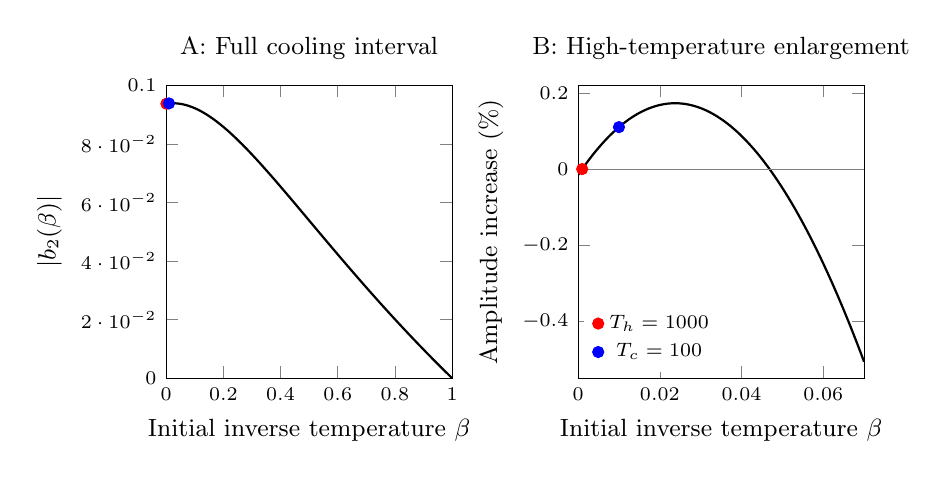
\begin{tikzpicture}
\begin{groupplot}[group style={group size=2 by 1,horizontal sep=1.6cm},width=0.43\textwidth,height=5.3cm,tick label style={font=\scriptsize},label style={font=\small},title style={font=\small},xlabel={Initial inverse temperature $\beta$},scaled ticks=false]
\nextgroupplot[title={A: Full cooling interval},xmin=0,xmax=1,ymin=0,ymax=.1,ylabel={$|b_2(\beta)|$}]
\addplot[black,thick] coordinates {(0,0.0937307280879) (0.008595988539,0.0938361114547) (0.01719197708,0.0938944479609) (0.02578796562,0.0939064820036) (0.03438395415,0.0938730351736) (0.04297994269,0.0937949992222) (0.05157593123,0.0936733290335) (0.06017191977,0.0935090356587) (0.06876790831,0.093303179468) (0.07736389685,0.0930568634644) (0.08595988539,0.0927712268026) (0.09455587393,0.0924474385483) (0.1031518625,0.0920866917064) (0.111747851,0.091690197544) (0.1203438395,0.0912591802263) (0.1289398281,0.0907948717793) (0.1375358166,0.0902985073893) (0.1461318052,0.0897713210442) (0.1547277937,0.0892145415173) (0.1633237822,0.0886293886924) (0.1719197708,0.088017070225) (0.1805157593,0.087378778531) (0.1891117479,0.0867156880944) (0.1977077364,0.0860289530815) (0.2063037249,0.085319705248) (0.2148997135,0.0845890521258) (0.223495702,0.0838380754735) (0.2320916905,0.0830678299749) (0.2406876791,0.0822793421697) (0.2492836676,0.0814736095994) (0.2578796562,0.0806516001538) (0.2664756447,0.0798142515995) (0.2750716332,0.0789624712781) (0.2836676218,0.0780971359555) (0.2922636103,0.0772190918105) (0.3008595989,0.0763291545473) (0.3094555874,0.0754281096185) (0.3180515759,0.0745167125467) (0.3266475645,0.0735956893329) (0.335243553,0.0726657369393) (0.3438395415,0.0717275238384) (0.3524355301,0.0707816906165) (0.3610315186,0.0698288506244) (0.3696275072,0.0688695906667) (0.3782234957,0.0679044717215) (0.3868194842,0.0669340296855) (0.3954154728,0.0659587761365) (0.4040114613,0.0649791991088) (0.4126074499,0.0639957638763) (0.4212034384,0.0630089137392) (0.4297994269,0.0620190708094) (0.4383954155,0.0610266367929) (0.446991404,0.0600319937636) (0.4555873926,0.0590355049289) (0.4641833811,0.058037515382) (0.4727793696,0.057038352841) (0.4813753582,0.0560383283716) (0.4899713467,0.0550377370939) (0.4985673352,0.0540368588702) (0.5071633238,0.0530359589736) (0.5157593123,0.0520352887381) (0.5243553009,0.0510350861871) (0.5329512894,0.0500355766425) (0.5415472779,0.049036973312) (0.5501432665,0.0480394778568) (0.558739255,0.047043280937) (0.5673352436,0.0460485627376) (0.5759312321,0.0450554934736) (0.5845272206,0.0440642338746) (0.5931232092,0.0430749356501) (0.6017191977,0.0420877419348) (0.6103151862,0.0411027877157) (0.6189111748,0.0401202002396) (0.6275071633,0.0391400994034) (0.6361031519,0.0381625981269) (0.6446991404,0.0371878027077) (0.6532951289,0.0362158131611) (0.6618911175,0.035246723543) (0.670487106,0.0342806222577) (0.6790830946,0.0333175923518) (0.6876790831,0.0323577117925) (0.6962750716,0.0314010537338) (0.7048710602,0.0304476867682) (0.7134670487,0.0294976751673) (0.7220630372,0.0285510791088) (0.7306590258,0.0276079548935) (0.7392550143,0.0266683551503) (0.7478510029,0.0257323290311) (0.7564469914,0.0247999223954) (0.7650429799,0.0238711779861) (0.7736389685,0.0229461355949) (0.782234957,0.0220248322201) (0.7908309456,0.0211073022154) (0.7994269341,0.0201935774316) (0.8080229226,0.0192836873498) (0.8166189112,0.0183776592084) (0.8252148997,0.0174755181225) (0.8338108883,0.0165772871976) (0.8424068768,0.0156829876369) (0.8510028653,0.0147926388423) (0.8595988539,0.0139062585109) (0.8681948424,0.0130238627254) (0.8767908309,0.0121454660398) (0.8853868195,0.0112710815608) (0.893982808,0.0104007210243) (0.9025787966,0.00953439486783) (0.9111747851,0.00867211229882) (0.9197707736,0.00781388135965) (0.9283667622,0.0069597089885) (0.9369627507,0.00610960107717) (0.9455587393,0.00526356252561) (0.9541547278,0.00442159729348) (0.9627507163,0.00358370844877) (0.9713467049,0.00274989821385) (0.9799426934,0.00192016800883) (0.9885386819,0.00109451849265) (0.9971346705,0.000272949601771) (1,1.2910072431e-80)};
\addplot[only marks,red,mark=*] coordinates {(.001,.0937454279941)};
\addplot[only marks,blue,mark=*] coordinates {(.01,.0938488356221)};
\nextgroupplot[title={B: High-temperature enlargement},xmin=0,xmax=.07,xtick={0,.02,.04,.06},xticklabel style={/pgf/number format/fixed,/pgf/number format/precision=2},ymin=-.55,ymax=.22,ylabel={Amplitude increase (\%)},legend style={font=\scriptsize,draw=none,at={(.02,.02)},anchor=south west}]
\addplot[black,thick,forget plot] coordinates {(0,-0.0156806646424) (0.000562248996,-0.00677952456806) (0.001124497992,0.00190404580884) (0.001686746988,0.0103702331446) (0.002248995984,0.018619225856) (0.00281124498,0.0266512141114) (0.003373493976,0.0344663898221) (0.003935742972,0.0420649466338) (0.004497991968,0.0494470799176) (0.005060240964,0.0566129867615) (0.00562248996,0.0635628659613) (0.006184738956,0.0702969180123) (0.006746987952,0.0768153451) (0.007309236948,0.0831183510916) (0.007871485944,0.0892061415273) (0.00843373494,0.0950789236112) (0.008995983936,0.100736906202) (0.009558232932,0.106180299807) (0.01012048193,0.111409316567) (0.01068273092,0.116424170254) (0.01124497992,0.121225076261) (0.01180722892,0.125812251588) (0.01236947791,0.130185914841) (0.01293172691,0.134346286216) (0.0134939759,0.138293587494) (0.0140562249,0.142028042032) (0.0146184739,0.145549874752) (0.01518072289,0.148859312135) (0.01574297189,0.151956582208) (0.01630522088,0.15484191454) (0.01686746988,0.157515540229) (0.01742971888,0.159977691894) (0.01799196787,0.162228603667) (0.01855421687,0.164268511185) (0.01911646586,0.166097651579) (0.01967871486,0.167716263463) (0.02024096386,0.169124586931) (0.02080321285,0.170322863542) (0.02136546185,0.171311336317) (0.02192771084,0.172090249723) (0.02248995984,0.17265984967) (0.02305220884,0.173020383499) (0.02361445783,0.173172099973) (0.02417670683,0.173115249269) (0.02473895582,0.17285008297) (0.02530120482,0.172376854053) (0.02586345382,0.171695816882) (0.02642570281,0.170807227198) (0.02698795181,0.169711342112) (0.0275502008,0.168408420095) (0.0281124498,0.166898720967) (0.0286746988,0.165182505889) (0.02923694779,0.163260037358) (0.02979919679,0.161131579191) (0.03036144578,0.158797396522) (0.03092369478,0.156257755789) (0.03148594378,0.153512924727) (0.03204819277,0.150563172361) (0.03261044177,0.147408768991) (0.03317269076,0.144049986189) (0.03373493976,0.140487096787) (0.03429718876,0.136720374869) (0.03485943775,0.132750095761) (0.03542168675,0.128576536025) (0.03598393574,0.124199973444) (0.03654618474,0.119620687021) (0.03710843373,0.114838956963) (0.03767068273,0.109855064677) (0.03823293173,0.104669292758) (0.03879518072,0.0992819249809) (0.03935742972,0.0936932462927) (0.03991967871,0.0879035428024) (0.04048192771,0.0819131017723) (0.04104417671,0.0757222116093) (0.0416064257,0.0693311618559) (0.0421686747,0.0627402431815) (0.04273092369,0.0559497473733) (0.04329317269,0.0489599673275) (0.04385542169,0.0417711970405) (0.04441767068,0.0343837316002) (0.04497991968,0.0267978671768) (0.04554216867,0.0190139010143) (0.04610441767,0.0110321314216) (0.04666666667,0.00285285776347) (0.04722891566,-0.00552361954771) (0.04779116466,-0.0140969990613) (0.04835341365,-0.0228669782967) (0.04891566265,-0.0318332537526) (0.04947791165,-0.0409955209151) (0.05004016064,-0.050353474267) (0.05060240964,-0.0599068072963) (0.05116465863,-0.0696552125048) (0.05172690763,-0.079598381417) (0.05228915663,-0.0897360045884) (0.05285140562,-0.100067771615) (0.05341365462,-0.110593371141) (0.05397590361,-0.121312490867) (0.05453815261,-0.132224817561) (0.05510040161,-0.143330037065) (0.0556626506,-0.154627834303) (0.0562248996,-0.166117893292) (0.05678714859,-0.177799897148) (0.05734939759,-0.189673528097) (0.05791164659,-0.201738467481) (0.05847389558,-0.213994395769) (0.05903614458,-0.226440992562) (0.05959839357,-0.239077936608) (0.06016064257,-0.251904905801) (0.06072289157,-0.264921577198) (0.06128514056,-0.278127627025) (0.06184738956,-0.291522730681) (0.06240963855,-0.305106562752) (0.06297188755,-0.318878797018) (0.06353413655,-0.332839106459) (0.06409638554,-0.346987163266) (0.06465863454,-0.361322638848) (0.06522088353,-0.375845203842) (0.06578313253,-0.390554528117) (0.06634538153,-0.405450280787) (0.06690763052,-0.420532130219) (0.06746987952,-0.435799744036) (0.06803212851,-0.451252789132) (0.06859437751,-0.466890931676) (0.06915662651,-0.482713837121) (0.0697188755,-0.498721170213) (0.07,-0.506793892168)};
\addplot[gray,forget plot] coordinates {(0,0)(.07,0)};
\addplot[only marks,red,mark=*] coordinates {(.001,0)};\addlegendentry{$T_h=1000$}
\addplot[only marks,blue,mark=*] coordinates {(.01,.1103068468)};\addlegendentry{$T_c=100$}
\end{groupplot}
\end{tikzpicture}
\caption{Thermal overlap of the exact primary generator, with $w_1=1$ and $T_b=1$. The broad curve conceals a small high-temperature maximum; the enlargement displays it. The blue preparation has a larger slow amplitude than the hotter red preparation. The enlarged ordinate uses the hot amplitude as its reference; the quoted 0.1102\% reduction uses the cold amplitude. Numerical curves use 80-digit arithmetic; the two selected overlaps are independently certified exactly.}
\label{fig:overlap}
\end{figure}


Initially $D_h(0)\simeq1.210137886$ and $D_c(0)\simeq1.155489557$, so the hotter preparation is farther away in relative entropy. The two distances cross numerically near $t=0.14967233$. Exact rational bounds prove a crossing in $(0.14,0.16)$: at the endpoints,
\begin{align*}
D_h(0.14)-D_c(0.14)&\in(5.9361291891,5.9361291893)\,10^{-8},\\
D_h(0.16)-D_c(0.16)&\in(-1.3100324358,-1.3100324356)\,10^{-8}.
\end{align*}
Total variation also reverses, with a certified crossing in $(0.10,0.11)$ and numerical location $0.10436410$. The difference between these times is expected: finite-time crossings depend on the distance. Continuity plus the certified signs proves existence; no uniqueness or earliest-crossing theorem is asserted.

\begin{figure}[htbp]
\centering
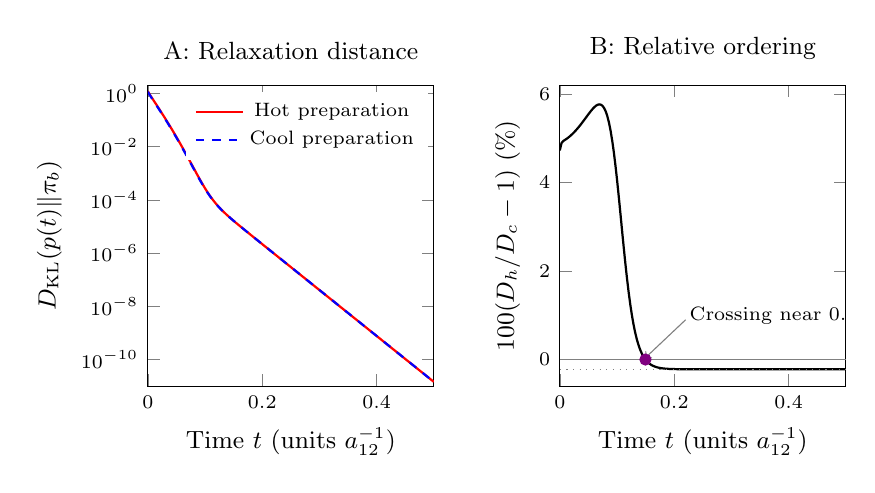
\begin{tikzpicture}
\begin{groupplot}[group style={group size=2 by 1,horizontal sep=1.6cm},width=0.43\textwidth,height=5.4cm,tick label style={font=\scriptsize},label style={font=\small},title style={font=\small},xlabel={Time $t$ (units $a_{12}^{-1}$)},xmin=0,xmax=.5]
\nextgroupplot[title={A: Relaxation distance},ymode=log,ymin=1e-11,ymax=2,ytick={1,1e-2,1e-4,1e-6,1e-8,1e-10},ylabel={$D_{\rm KL}(p(t)\Vert\pi_b)$},legend style={font=\scriptsize,draw=none,at={(.98,.98)},anchor=north east}]
\addplot[red,thick] coordinates {(0,1.21013788612) (0.004297994269,0.842995461777) (0.008595988539,0.608987398936) (0.01289398281,0.440341581659) (0.01719197708,0.317610499322) (0.02148997135,0.228359408254) (0.02578796562,0.163590181022) (0.03008595989,0.116712896394) (0.03438395415,0.0828931212786) (0.03868194842,0.0585837956434) (0.04297994269,0.0411839769259) (0.04727793696,0.0287887239354) (0.05157593123,0.0200052178145) (0.0558739255,0.0138173290506) (0.06017191977,0.0094857680391) (0.06446991404,0.00647444487958) (0.06876790831,0.00439616683326) (0.07306590258,0.00297261554659) (0.07736389685,0.00200487053096) (0.08166189112,0.00135171854244) (0.08595988539,0.000913707520456) (0.09025787966,0.000621437483811) (0.09455587393,0.000426978003437) (0.09885386819,0.000297596870429) (0.1031518625,0.000211201716764) (0.1074498567,0.000153053858448) (0.111747851,0.000113426372608) (0.1160458453,8.59590776246e-05) (0.1203438395,6.65220464343e-05) (0.1246418338,5.24440941518e-05) (0.1289398281,4.19979987345e-05) (0.1332378223,3.40624669361e-05) (0.1375358166,2.79032297638e-05) (0.1418338109,2.30328834405e-05) (0.1461318052,1.91219036217e-05) (0.1504297994,1.59424477581e-05) (0.1547277937,1.33329329201e-05) (0.159025788,1.11756708466e-05) (0.1633237822,9.38266728223e-06) (0.1676217765,7.88651546087e-06) (0.1719197708,6.63447149767e-06) (0.176217765,5.58452620241e-06) (0.1805157593,4.70273986701e-06) (0.1848137536,3.96138595297e-06) (0.1891117479,3.33762156401e-06) (0.1934097421,2.81250823938e-06) (0.1977077364,2.37027154024e-06) (0.2020057307,1.99772792466e-06) (0.2063037249,1.68383221109e-06) (0.2106017192,1.41931443341e-06) (0.2148997135,1.19638469923e-06) (0.2191977077,1.00849096794e-06) (0.223495702,8.50118800469e-07) (0.2277936963,7.1662491024e-07) (0.2320916905,6.040982621e-07) (0.2363896848,5.09243827335e-07) (0.2406876791,4.292850983e-07) (0.2449856734,3.61882214057e-07) (0.2492836676,3.05063124171e-07) (0.2535816619,2.57165670569e-07) (0.2578796562,2.16788829415e-07) (0.2621776504,1.82751648505e-07) (0.2664756447,1.5405865608e-07) (0.270773639,1.29870715468e-07) (0.2750716332,1.09480464761e-07) (0.2793696275,9.22916181458e-08) (0.2836676218,7.78015204764e-08) (0.287965616,6.55864430043e-08) (0.2922636103,5.52891890983e-08) (0.2965616046,4.66086467801e-08) (0.3008595989,3.92909821095e-08) (0.3051575931,3.31222156051e-08) (0.3094555874,2.79219644352e-08) (0.3137535817,2.35381672681e-08) (0.3180515759,1.984263745e-08) (0.3223495702,1.67273144245e-08) (0.3266475645,1.41011037445e-08) (0.3309455587,1.18872132503e-08) (0.335243553,1.00209075023e-08) (0.3395415473,8.44761479409e-09) (0.3438395415,7.12133138393e-09) (0.3481375358,6.00327627651e-09) (0.3524355301,5.06075721525e-09) (0.3567335244,4.26621472219e-09) (0.3610315186,3.59641623017e-09) (0.3653295129,3.03177674123e-09) (0.3696275072,2.5557861454e-09) (0.3739255014,2.1545264534e-09) (0.3782234957,1.81626482611e-09) (0.38252149,1.53111050007e-09) (0.3868194842,1.29072557705e-09) (0.3911174785,1.08808122076e-09) (0.3954154728,9.17252131338e-10) (0.399713467,7.73243288105e-10) (0.4040114613,6.51843894075e-10) (0.4083094556,5.49504251606e-10) (0.4126074499,4.63231968835e-10) (0.4169054441,3.90504461927e-10) (0.4212034384,3.29195194641e-10) (0.4255014327,2.77511498414e-10) (0.4297994269,2.33942154795e-10) (0.4340974212,1.9721320751e-10) (0.4383954155,1.66250712102e-10) (0.4426934097,1.40149333914e-10) (0.446991404,1.18145876234e-10) (0.4512893983,9.95969645406e-11) (0.4555873926,8.39602343497e-11) (0.4598853868,7.07784725827e-11) (0.4641833811,5.96662487535e-11) (0.4684813754,5.02986450691e-11) (0.4727793696,4.24017559113e-11) (0.4770773639,3.57446789062e-11) (0.4813753582,3.01327634e-11) (0.4856733524,2.54019189279e-11) (0.4899713467,2.14138172552e-11) (0.494269341,1.80518477013e-11) (0.4985673352,1.52177074778e-11) (0.5,1.43755705045e-11)};\addlegendentry{Hot preparation}
\addplot[blue,dashed,thick] coordinates {(0,1.1554895572) (0.004297994269,0.803461576189) (0.008595988539,0.580185474244) (0.01289398281,0.419364575234) (0.01719197708,0.302354194621) (0.02148997135,0.217286688894) (0.02578796562,0.155575093154) (0.03008595989,0.110929645075) (0.03438395415,0.0787358757628) (0.03868194842,0.0556082906007) (0.04297994269,0.0390647635126) (0.04727793696,0.0272877691897) (0.05157593123,0.0189487897175) (0.0558739255,0.0130789599167) (0.06017191977,0.00897369130476) (0.06446991404,0.00612233088008) (0.06876790831,0.00415629420604) (0.07306590258,0.00281084148171) (0.07736389685,0.00189692923778) (0.08166189112,0.00128049982498) (0.08595988539,0.000867258167281) (0.09025787966,0.000591495738387) (0.09455587393,0.000407901651071) (0.09885386819,0.000285582655926) (0.1031518625,0.000203720946556) (0.1074498567,0.000148448546014) (0.111747851,0.000110624197399) (0.1160458453,8.42754713897e-05) (0.1203438395,6.55252253156e-05) (0.1246418338,5.18646974948e-05) (0.1289398281,4.16696612046e-05) (0.1332378223,3.38833734381e-05) (0.1375358166,2.78116075661e-05) (0.1418338109,2.29915772606e-05) (0.1461318052,1.91087726656e-05) (0.1504297994,1.59444421841e-05) (0.1547277937,1.3342468424e-05) (0.159025788,1.11884247183e-05) (0.1633237822,9.39624667441e-06) (0.1676217765,7.89965729757e-06) (0.1719197708,6.64656461516e-06) (0.176217765,5.59532783414e-06) (0.1805157593,4.71220880055e-06) (0.1848137536,3.96958540287e-06) (0.1891117479,3.34466348692e-06) (0.1934097421,2.81852213046e-06) (0.1977077364,2.37538757317e-06) (0.2020057307,2.00206840073e-06) (0.2063037249,1.68750774255e-06) (0.2106017192,1.42242275658e-06) (0.2148997135,1.19901088906e-06) (0.2191977077,1.01070834563e-06) (0.223495702,8.51990133239e-07) (0.2277936963,7.18203682565e-07) (0.2320916905,6.05429902655e-07) (0.2363896848,5.10366836116e-07) (0.2406876791,4.30232052248e-07) (0.2449856734,3.62680647913e-07) (0.2492836676,3.05736292829e-07) (0.2535816619,2.57733203551e-07) (0.2578796562,2.17267289645e-07) (0.2621776504,1.83155007565e-07) (0.2664756447,1.54398697361e-07) (0.270773639,1.30157375524e-07) (0.2750716332,1.0972212196e-07) (0.2793696275,9.24953365351e-08) (0.2836676218,7.79732556769e-08) (0.287965616,6.57312159652e-08) (0.2922636103,5.54112326839e-08) (0.2965616046,4.67115294085e-08) (0.3008595989,3.9377712018e-08) (0.3051575931,3.31953287689e-08) (0.3094555874,2.7983598696e-08) (0.3137535817,2.35901248321e-08) (0.3180515759,1.98864375779e-08) (0.3223495702,1.67642378516e-08) (0.3266475645,1.41322301285e-08) (0.3309455587,1.19134527402e-08) (0.335243553,1.00430273512e-08) (0.3395415473,8.46626179447e-09) (0.3438395415,7.13705077999e-09) (0.3481375358,6.01652770769e-09) (0.3524355301,5.0719281564e-09) (0.3567335244,4.27563181367e-09) (0.3610315186,3.60435482906e-09) (0.3653295129,3.03846897295e-09) (0.3696275072,2.56142769121e-09) (0.3739255014,2.15928227225e-09) (0.3782234957,1.82027397811e-09) (0.38252149,1.53449021265e-09) (0.3868194842,1.2935746728e-09) (0.3911174785,1.09048300697e-09) (0.3954154728,9.19276835952e-10) (0.399713467,7.74950113201e-10) (0.4040114613,6.53282746945e-10) (0.4083094556,5.50717204048e-10) (0.4126074499,4.64254487339e-10) (0.4169054441,3.91366444716e-10) (0.4212034384,3.29921845895e-10) (0.4255014327,2.7812406524e-10) (0.4297994269,2.34458548491e-10) (0.4340974212,1.9764852729e-10) (0.4383954155,1.66617686596e-10) (0.4426934097,1.40458693352e-10) (0.446991404,1.18406666193e-10) (0.4512893983,9.98168104413e-11) (0.4555873926,8.41455644174e-11) (0.4598853868,7.09347058098e-11) (0.4641833811,5.97979533491e-11) (0.4684813754,5.0409672032e-11) (0.4727793696,4.24953516327e-11) (0.4770773639,3.58235800932e-11) (0.4813753582,3.01992770962e-11) (0.4856733524,2.54579899704e-11) (0.4899713467,2.14610851417e-11) (0.494269341,1.80916945279e-11) (0.4985673352,1.52512983514e-11) (0.5,1.44073024831e-11)};\addlegendentry{Cool preparation}
\nextgroupplot[title={B: Relative ordering},ylabel={$100(D_h/D_c-1)$ (\%)},ymin=-.6,ymax=6.2]
\addplot[black,thick] coordinates {(0,4.72945242796) (0.002865329513,4.89158842429) (0.005730659026,4.93838902716) (0.008595988539,4.96426159744) (0.01146131805,4.98892905107) (0.01432664756,5.01595684521) (0.01719197708,5.04583861343) (0.02005730659,5.07853498975) (0.0229226361,5.11393161062) (0.02578796562,5.15190941246) (0.02865329513,5.19234463846) (0.03151862464,5.23509603344) (0.03438395415,5.27998891932) (0.03724928367,5.32679719851) (0.04011461318,5.37522281625) (0.04297994269,5.42487198877) (0.04584527221,5.4752275317) (0.04871060172,5.52561674363) (0.05157593123,5.57517452435) (0.05444126074,5.62280178951) (0.05730659026,5.66711985913) (0.06017191977,5.70642244031) (0.06303724928,5.73862820073) (0.0659025788,5.76123884197) (0.06876790831,5.77131009811) (0.07163323782,5.76544617307) (0.07449856734,5.73983155693) (0.07736389685,5.69031733132) (0.08022922636,5.61258084449) (0.08309455587,5.50237615175) (0.08595988539,5.35588535542) (0.0888252149,5.17016528956) (0.09169054441,4.94365846468) (0.09455587393,4.67670388594) (0.09742120344,4.3719502183) (0.100286533,4.03455512448) (0.1031518625,3.67206727382) (0.106017192,3.29394163068) (0.1088825215,2.91072690005) (0.111747851,2.53305811393) (0.1146131805,2.1706483271) (0.11747851,1.8314729471) (0.1203438395,1.52127842967) (0.1232091691,1.24345246791) (0.1260744986,0.999204660263) (0.1289398281,0.787953442396) (0.1318051576,0.607803886449) (0.1346704871,0.456021168678) (0.1375358166,0.329438697433) (0.1404011461,0.224773429427) (0.1432664756,0.138845874155) (0.1461318052,0.0687168997329) (0.1489971347,0.011759483314) (0.1518624642,-0.0343160525548) (0.1547277937,-0.0714673148158) (0.1575931232,-0.101343199991) (0.1604584527,-0.125316431572) (0.1633237822,-0.144519324029) (0.1661891117,-0.159879081081) (0.1690544413,-0.172150543859) (0.1719197708,-0.18194538362) (0.1747851003,-0.18975741719) (0.1776504298,-0.195984128036) (0.1805157593,-0.200944693858) (0.1833810888,-0.20489492013) (0.1862464183,-0.208039504929) (0.1891117479,-0.210542045055) (0.1919770774,-0.212533156905) (0.1948424069,-0.214117040194) (0.1977077364,-0.215376765843) (0.2005730659,-0.216378524956) (0.2034383954,-0.217175035928) (0.2063037249,-0.217808271964) (0.2091690544,-0.218311641636) (0.212034384,-0.218711730305) (0.2148997135,-0.219029689635) (0.217765043,-0.219282345544) (0.2206303725,-0.219483081147) (0.223495702,-0.219642540063) (0.2263610315,-0.219769186431) (0.229226361,-0.219869750693) (0.2320916905,-0.219949584356) (0.2349570201,-0.220012942266) (0.2378223496,-0.22006320717) (0.2406876791,-0.220103068339) (0.2435530086,-0.220134663631) (0.2464183381,-0.22015969248) (0.2492836676,-0.22017950574) (0.2521489971,-0.220195177131) (0.2550143266,-0.220207560044) (0.2578796562,-0.220217332713) (0.2607449857,-0.220225034124) (0.2636103152,-0.220231092572) (0.2664756447,-0.220235848355) (0.2693409742,-0.220239571828) (0.2722063037,-0.220242477746) (0.2750716332,-0.220244736672) (0.2779369628,-0.220246484044) (0.2808022923,-0.220247827385) (0.2836676218,-0.220248852033) (0.2865329513,-0.220249625696) (0.2893982808,-0.220250202072) (0.2922636103,-0.22025062373) (0.2951289398,-0.220250924397) (0.2979942693,-0.220251130777) (0.3008595989,-0.220251263996) (0.3037249284,-0.22025134075) (0.3065902579,-0.220251374221) (0.3094555874,-0.220251374801) (0.3123209169,-0.220251350667) (0.3151862464,-0.220251308242) (0.3180515759,-0.220251252559) (0.3209169054,-0.220251187546) (0.323782235,-0.220251116263) (0.3266475645,-0.220251041076) (0.329512894,-0.220250963809) (0.3323782235,-0.220250885855) (0.335243553,-0.220250808268) (0.3381088825,-0.220250731836) (0.340974212,-0.220250657136) (0.3438395415,-0.220250584586) (0.3467048711,-0.220250514471) (0.3495702006,-0.220250446981) (0.3524355301,-0.220250382226) (0.3553008596,-0.220250320261) (0.3581661891,-0.220250261093) (0.3610315186,-0.220250204697) (0.3638968481,-0.220250151022) (0.3667621777,-0.2202501) (0.3696275072,-0.220250051549) (0.3724928367,-0.220250005577) (0.3753581662,-0.22024996199) (0.3782234957,-0.220249920688) (0.3810888252,-0.22024988157) (0.3839541547,-0.220249844537) (0.3868194842,-0.220249809489) (0.3896848138,-0.220249776329) (0.3925501433,-0.220249744964) (0.3954154728,-0.220249715303) (0.3982808023,-0.220249687258) (0.4011461318,-0.220249660744) (0.4040114613,-0.220249635681) (0.4068767908,-0.220249611993) (0.4097421203,-0.220249589605) (0.4126074499,-0.220249568448) (0.4154727794,-0.220249548456) (0.4183381089,-0.220249529564) (0.4212034384,-0.220249511714) (0.4240687679,-0.220249494849) (0.4269340974,-0.220249478915) (0.4297994269,-0.22024946386) (0.4326647564,-0.220249449636) (0.435530086,-0.220249436199) (0.4383954155,-0.220249423504) (0.441260745,-0.220249411511) (0.4441260745,-0.220249400181) (0.446991404,-0.220249389478) (0.4498567335,-0.220249379366) (0.452722063,-0.220249369814) (0.4555873926,-0.22024936079) (0.4584527221,-0.220249352265) (0.4613180516,-0.220249344212) (0.4641833811,-0.220249336604) (0.4670487106,-0.220249329418) (0.4699140401,-0.220249322629) (0.4727793696,-0.220249316215) (0.4756446991,-0.220249310157) (0.4785100287,-0.220249304434) (0.4813753582,-0.220249299027) (0.4842406877,-0.22024929392) (0.4871060172,-0.220249289095) (0.4899713467,-0.220249284537) (0.4928366762,-0.220249280232) (0.4957020057,-0.220249276164) (0.4985673352,-0.220249272322) (0.5,-0.220249270481)};
\addplot[gray] coordinates {(0,0)(.5,0)};
\addplot[gray,dotted] coordinates {(0,-.2202492067)(.5,-.2202492067)};
\addplot[only marks,violet,mark=*] coordinates {(.1496723312,0)};
\node[font=\scriptsize,anchor=west] at (axis cs:.21,1) {Crossing near $0.14967$};
\draw[->,gray] (axis cs:.22,.9) -- (axis cs:.1496723312,.04);
\end{groupplot}
\end{tikzpicture}
\caption{Actual evolution $p(t)=e^{tM}\pi(\beta)$ for the same two preparations. Relative entropy decreases for each, and the hotter state's distance becomes smaller. The ratio panel resolves the crossing that is difficult to see on the logarithmic plot. The horizontal dotted line is the asymptotic ratio difference, $-0.2202492\%$. Rational uniformization and logarithm bounds certify opposite KL orderings at $t=0.14$ and $0.16$; the displayed root location is numerical, with no claim of uniqueness.}
\label{fig:crossing}
\end{figure}


The relevant fractional amplitude reduction is
\[
\epsilon_b=1-\frac{|b_h|}{|b_c|}\simeq0.0011018531=0.11018531\%.
\]
For relative entropy the leading term is quadratic, so
\[
1-\lim_{t\to\infty}\frac{D_h(t)}{D_c(t)}
=1-\frac{b_h^2}{b_c^2}\simeq0.22024921\%.
\]
Both preparations have the same decay exponent $\lambda_2$. This is an ordinary effect, not the exponentially faster strong effect. For an increasingly small common distance threshold, the asymptotic time advance is
\[
\Delta t=\frac{\log(|b_c|/|b_h|)}{|\lambda_2|}
\simeq5.5488\,10^{-5}\,a_{12}^{-1}.
\]
The slow relaxation time is $1/|\lambda_2|\simeq0.0503313\,a_{12}^{-1}$, so this advance is only about $0.11025\%$ of one slow relaxation time. It is not a percentage reduction in the full cooling time, which depends on the chosen threshold. The time unit has no assigned experimental value, and $T_h/T_b=1000$, $T_c/T_b=100$. These data establish a strict mathematical failure of the triplet inference; they do not establish a practically useful cooling protocol.

\subsection{A corrected sufficient condition}
Let $L=M^\top$ act on functions, $(Lf)_i=\sum_{j\ne i}a_{ji}(f_j-f_i)$. Define adjacent differences $y_i=f_{i+1}-f_i$, the difference map $Bf=y$, and $(H_0y)_j=\sum_{\ell<j}y_\ell$. Then $BL=KB$ with $K=BLH_0$, since $L\mathbf1=0$. In the constant-plus-differences basis, $L$ is block triangular with blocks 0 and $K$, so $K$ has precisely the nonzero generator eigenvalues. For its off-diagonal entries,
\[
K_{i\ell}=\begin{cases}
\sum_{j\leq\ell}(a_{j,i}-a_{j,i+1}),&\ell<i,\\
\sum_{j>\ell}(a_{j,i+1}-a_{j,i}),&\ell>i.
\end{cases}
\]
\begin{theorem}[Order-preserving sufficient condition]
For any finite number of states, strictly ordered energies, a fixed $0<\beta_b<\infty$, positive reversible rates and a simple slowest nonzero eigenvalue, if every off-diagonal entry of $K$ is nonnegative, there is no asymptotic cooling or heating Mpemba effect at positive initial temperatures.
\end{theorem}
\begin{proof}
Such a matrix $K$ is called Metzler. After a sufficiently large scalar diagonal shift it is nonnegative. Perron theory gives a nonzero nonnegative eigenvector $y$ at its spectral abscissa, which is $\lambda_2$. This does not require irreducibility of $K$. Choose $w$ with $Bw=y$ and $\pi_b^\top w=0$. Then $B(Lw-\lambda_2w)=0$, so $Lw-\lambda_2w$ is constant. Its bath expectation is zero, hence it vanishes. Thus $w$ is the slow left eigenfunction, nondecreasing and nonconstant in energy.

The covariance identity now gives $b_2'(\beta)<0$ for every finite positive $\beta$: all its pairwise summands are nonnegative and at least one is strictly positive. Because $b_2(\beta_b)=0$, its absolute value decreases toward the bath on the cooling side and increases away from the bath on the heating side. These are exactly the normal asymptotic orderings.
\end{proof}
In four states, the six off-diagonal entries are
\begin{align*}
K_{12}&=a_{32}+a_{42}-a_{31}-a_{41},&K_{13}&=a_{42}-a_{41},\\
K_{21}&=a_{12}-a_{13},&K_{23}&=a_{43}-a_{42},\\
K_{31}&=a_{13}-a_{14},&K_{32}&=a_{13}+a_{23}-a_{14}-a_{24}.
\end{align*}
The original failures already ensure the three upper entries are nonnegative, since $G\leq0$ orders upward rates. A corrected, directly checkable sufficient condition is therefore the four original failures together with
\[
a_{12}\geq a_{13},\qquad a_{13}\geq a_{14},\qquad
 a_{13}+a_{23}\geq a_{14}+a_{24}.
\]
This is a proved sufficient condition, not a proposed necessary characterization.

\begin{corollary}
If every triplet has $\kappa\leq1$ and fails the original predicate, then the absence conclusion is true, for any state count under the theorem's assumptions.
\end{corollary}
\begin{proof}
$H\leq0$ and $G\leq0$ give $A+B\leq C(1+t)$ and $B\geq At$, so $A\leq C$. These comparisons make each downward summand in $K$ nonnegative; $G\leq0$ and detailed balance do the same for each upward summand. Apply the theorem.
\end{proof}
A second subfamily consists of downward gap laws $a_{ij}=f(E_j-E_i)$, $i<j$, with positive nonincreasing $f$. Both $f(x)$ and $e^{-\beta_bx}f(x)$ are nonincreasing, so every required summand is nonnegative. This establishes the same absence conclusion directly, without the false general triplet conjecture. The following comparison locates this argument within established order theory; no general monotonicity novelty is claimed.

\subsection{Relation to earlier no-Mpemba theorems}\label{sec:priororder}
\href{https://arxiv.org/html/2410.06623v2}{Ohga, Hayakawa and Ito (OHI), Result 2 and SI D} already use monotone coupling to exclude Mpemba behavior. Their SI D2 explicitly treats a total order. Our matrix condition is precisely a finite-chain expression of stochastic monotonicity, not a separate physical principle. The relevant distinctions are:
\begin{center}\small
\begin{tabular}{p{.17\textwidth}p{.36\textwidth}p{.36\textwidth}}
\toprule &OHI Result 2&The preceding spectral criterion\\\midrule
State order&Finite partial order; energy respects it&Total order by distinct energies\\
Dynamics&Irreducible and Gibbs-stationary; reversibility unnecessary&Positive reversible rates\\
Order condition&Comparable jumps and a monotone coupling&$K=BLH_0$ is Metzler\\
Bath range&Hypotheses throughout a temperature interval&One fixed finite positive bath\\
Spectrum&No simplicity requirement&Simple slowest nonzero eigenvalue\\
Conclusion&No cooling mean-energy crossing at any time&No asymptotic cooling/heating reversal in fixed norms or KL\\\bottomrule
\end{tabular}
\end{center}
OHI SI B extends their Result 1, the microscopic characterization, to KL divergence; it does not state Result 2 as an all-time KL theorem. Thus the different observable and time scopes must not be conflated.

Indeed $BL=KB$ gives $Be^{tL}=e^{tK}B$. The Metzler condition is equivalent to $e^{tL}$ preserving increasing functions: sufficiency follows from $e^{tK}\geq0$, and necessity by differentiation at zero on coordinate vectors of adjacent differences. This also gives a monotone coupling. Choose $r$ large enough that $I+L/r$ is stochastic and $I+K/r$ is entrywise nonnegative. Its transition rows are stochastically ordered. A common Poisson clock of rate $r$ and common-uniform inverse-CDF updates preserve the order of two copies. On a total order, energy compatibility and comparability of jumps are automatic.

For fixed bath, $e^{tL}E$ is then increasing, so
\[
\partial_\beta\{\pi(\beta)^\top e^{tL}E\}
=-\Cov_{\pi(\beta)}(e^{tL}E,E)\leq0.
\]
This gives all-time energy ordering without reversibility or spectral simplicity. It explains the direct relation to OHI while avoiding an inference from a single observable to all possible distances.

The likelihood-ratio and stochastic-order methods below also have precedent in \href{https://arxiv.org/abs/1109.6075}{Fill and Kahn, Ann. Appl. Probab. 23 (2013), 1778--1816}, particularly their comparison framework and Corollary 3.3. Their setup compares different kernels under suitable initial laws; the thermal preparations here differ instead. We provide the following consequence for clarity, without a priority claim.

\begin{corollary}[All-time divergence ordering under reversible monotonicity]
Let a finite irreducible generator be reversible with positive Gibbs equilibrium, on a total energy order, and let $K$ be Metzler. For any convex $\Phi$ finite on positive arguments, with $\Phi(1)=0$, define
\[
D_\Phi(p\Vert\pi_b)=\sum_i\pi_{bi}\Phi(p_i/\pi_{bi}).
\]
For same-side Gibbs preparations, the farther initial temperature has at least as large a divergence at every $t\geq0$. This includes KL and total variation, and requires no simple eigenvalue. For KL the inequality is strict at every finite time for distinct initial temperatures.
\end{corollary}
\begin{proof}
Write $p\succeq_{\rm st}q$ when $\sum_i p_i f_i\geq\sum_i q_i f_i$ for every increasing $f$. Gibbs laws are stochastically ordered by temperature, by the pairwise covariance identity. A monotone semigroup preserves this order. Thus for cooling $p_h(t)\succeq_{\rm st}p_c(t)\succeq_{\rm st}\pi_b$.

Reversibility implies $p_c(t)/\pi_b=e^{tL}[\pi(\beta_c)/\pi_b]$ componentwise. The initial ratio is proportional to $e^{(\beta_b-\beta_c)E_i}$ and is increasing; it stays increasing. Choose a nondecreasing subgradient $g$ of $\Phi$. Convexity and stochastic order give
\[
D_\Phi(p_h\Vert\pi_b)-D_\Phi(p_c\Vert\pi_b)
\geq\sum_i(p_{hi}-p_{ci})g(p_{ci}/\pi_{bi})\geq0.
\]
For heating, $p_c\preceq_{\rm st}p_h\preceq_{\rm st}\pi_b$ and $p_h/\pi_b$ is decreasing. Apply the same supporting-line inequality at $p_h/\pi_b$ to obtain $D_\Phi(p_c\Vert\pi_b)\geq D_\Phi(p_h\Vert\pi_b)$. KL is strictly convex, and invertibility of $e^{tM}$ keeps two distinct initial distributions distinct at finite $t$, proving strictness.
\end{proof}
This does not assert all-time ordering for every arbitrary norm. The original spectral proof supplies the every-fixed-norm conclusion asymptotically with a simple slow mode. Our counterexample violates monotonicity explicitly: $K_{21}=a_{12}-a_{13}=-27$. It therefore challenges neither OHI's theorem nor this corollary.

The defensible contribution claim is the exact counterexample to the unrestricted triplet inference, its robust family and mechanism, and the explicit triplet-rate connection to an established sufficient condition. We do not present the general order-preservation mechanism or the elementary divergence consequence as newly discovered principles. The all-$\kappa\leq1$ statement is an application; its broader publication priority remains unestablished.

\section{Approaches explored}
The initial route comparison, including explicit continue/change criteria, is recorded in \path{research/approaches.md}. The decisive work covered both theorem construction and adversarial falsification.
\begin{enumerate}
\item \textbf{Reversible spectral geometry.} Symmetrization and the Dirichlet form gave reliable eigenvalue ordering and an equilibrium-orthogonal search space. The obstacle was that rate inequalities do not make the slow-mode orientation convex. Spectral certificates remain essential; this route did not yield the full absence theorem.
\item \textbf{Order and covariance.} The first calculation was $K=BLH_0$. Its Metzler subfamily yielded the theorem above. An exact auxiliary example in \path{research/theorem_notes.md} disproves the intermediate claim that all triplet failures force a monotone slow eigenvector. This identified the missing implication rather than assuming it.
\item \textbf{Exponential-polynomial zero counting.} Multiplying by $Z(\beta)^2$ gives
\[
Z^2b_2'=-\sum_{i<j}(w_j-w_i)(E_j-E_i)e^{-\beta(E_i+E_j)}.
\]
For four states there are at most six distinct exponential terms. Chebyshev/variation arguments could bound turning points, but cannot exclude the certified turning behavior. No new general zero-count theorem is claimed. This route became explanatory, not decisive.
\item \textbf{Feasible-rate geometry.} The identity $F=hG+dH$ converted apparent branch enumeration into eight linear inequalities. A search enumerated extremal rays after removing the reset direction, then sampled positive mixtures. It found the first root-search candidate after 67,000 systems. Extremal rays were used for discovery only: we did not assume eigenvector properties are inherited by mixtures.
\item \textbf{Backward eigenvector design.} Starting from the discovered thermal mode, we prescribed rational $q$ and rational $w$ with $q^\top w=0$, then solved the linear eigenvector equations for rates. This produced the rational-mode companion and an exact eigenvalue. The remaining spectrum was checked independently; realization of an arbitrary faster eigenmode would not suffice.
\item \textbf{Lumping and perturbation.} The near-neutral highest state explains the observed mode. No adiabatically eliminated rate was substituted into the original predicate. Strict-margin continuity supplies a rigorous open family; a separate singular-perturbation theorem was unnecessary once a finite positive example was certified.
\item \textbf{Difficult regimes and targeted sampling.} Broad positive-rate sampling missed the effect. Signed-cone directions plus reset restoration found an independent witness. This concentrated the search on unequal energy gaps and narrow high-temperature windows, where a coarse temperature grid is weak.
\item \textbf{Algebraic proof.} Rational bath weights made the selected Gibbs probabilities algebraic even though the energy gaps are not commensurate. Exact root brackets and rational interval arithmetic proved the two-temperature inequality. Commensurate energies were therefore not needed.
\item \textbf{Additional idea: reset lineality.} The reset generator lies in the lineality space of all the triplet inequalities and acts as a scalar on nonstationary modes. This allowed signed directions to be made physical without changing their mode geometry, and gives the explicit counterexample family above. The September paper also studies the fully degenerate reset point; general novelty of that point is not claimed.
\item \textbf{Additional idea: thermal dual cones.} The cone spanned by Gibbs tangent vectors would have a dual consisting of modes with controlled derivative sign. The first calculation was the covariance expansion. The counterexample shows that the original rate cone's slow modes cross the required thermal dual. A complete dual-cone characterization remains an extension, not a premise used in the proof.
\end{enumerate}

\section{Verification and reproducibility}
\subsection{Exact certificate construction}
Run from the workspace root:
\begin{verbatim}
python3 research/adversarial_certificate.py
python3 research/adversarial_rational_mode_certificate.py
\end{verbatim}
The primary script uses SymPy rational/integer arithmetic to check positivity, column sums, detailed balance and the original Boolean predicates. It derives the characteristic polynomial and cofactor vector and verifies its eigenvector residual and bath expectation modulo $C(x)$. The actual slow root is enclosed between
\[
-\frac{42820190741029}{2155193997917}
\quad\hbox{and}\quad
-\frac{135549509489200}{6822377112669}.
\]
Opposite exact polynomial signs certify this interval. Two disjoint negative intervals similarly contain the other roots; degree three proves completeness. The interval evaluation of $P_1$ excludes zero, so division by it is justified.

For each $q_i^{1/n}$, $n=1000,100$, the script proposes adjacent grid points $L_i,U_i$ of mesh $10^{-24}$, then checks exactly
\[
0\leq L_i,\qquad L_i^n\leq q_i\leq U_i^n.
\]
Strict monotonicity of the positive $n$th-power map proves the enclosure. Approximate arithmetic only proposes the endpoints; it never accepts an inequality. Polynomial Horner evaluation, products and division use exact interval endpoints. All denominators are verified to exclude zero. The final interval comparison is also exact. Full rational endpoints, rather than merely rounded decimals, are saved in the JSON certificates.

The tighter certified margin in the primary normalization is greater than
\[0.00010340762800011847331527.\]
The deliberately widened report bounds are conservative. Scaling $w$ consistently changes the displayed numbers but never the conclusion; search logs may use a unit weighted norm, whereas the final report fixes $w_1=1$.

\subsection{Figure and finite-time verification}
Run \path{research/physics_plots.py} for the figures and data, and \path{research/finite_time_certificate.py} for exact finite-time bounds. Plot values use 80-digit mpmath arithmetic. Direct matrix exponentiation and reversible symmetric spectral propagation agree within $6\,10^{-81}$ at ten checks spanning $t=0$ to $0.4$. The plot CSV files and numerical metrics are saved under \path{output/figures/}. Those numerical comparisons are distinct from the exact certificates.

The finite-time certificate uses uniformization with $\nu=253$ and the exactly stochastic matrix $P=I+M/\nu$:
\[
e^{tM}p(0)=e^{-\nu t}\sum_{k=0}^{\infty}\frac{(\nu t)^k}{k!}P^kp(0).
\]
It retains terms through $k=250$. Each omitted probability component is at most one; the scalar positive-series tail is bounded by its first omitted term divided by $1-\nu t/252$. The same positive Taylor bounds give a rational enclosure of $e^{-\nu t}$. Initial Gibbs probabilities use the already-certified algebraic brackets. For logarithms it uses
\[
\log r=2\sum_{k=0}^{59}\frac{z^{2k+1}}{2k+1}+R,
\quad z=\frac{r-1}{r+1},\quad
|R|\leq\frac{2|z|^{121}}{121(1-z^2)}.
\]
All interval operations round outward onto a rational grid of mesh $10^{-50}$. Exact rational endpoint signs prove the displayed KL and TV crossing brackets. The script uses floating point only to print readable values. The root estimates shown on the figures are numerical; their enclosing crossing intervals are exact.

\subsection{Executed discovery calculations}
The discovery environment used Python with NumPy 1.26.4, SciPy 1.13.1 and SymPy 1.14.0. Seeds and actual parameters are retained in the scripts and output files. Floating-point discovery outputs are not mathematical certificates.

\path{research/cone_search.py} used seed 10411, energy gaps $\exp U[-4,2]$, 1,000 ray mixtures per energy set, and 150 cooling inverse temperatures from 0.001 to 0.999. It stopped after 67 energy sets, 67,000 systems, on a strict candidate. Coefficients of the ray mixtures were $\exp U[-9,3]$; a reset direction restored positivity. SVD acceptance tolerances for rays were $10^{-8}$ and $10^{-9}$, and deduplication tolerance $10^{-6}$. These are discovery tolerances only.

The independent positive-rate search used seed 934256 and 20,000,000 draws. Gaps were $10^{U[-3,1]}$, rates $10^{U[-5,5]}$ rescaled by their maximum; 2,020,118 draws passed the predicates. It found no accepted witness on its 18-point cooling/heating grid, under the margins and spectral filters in \path{research/adversarial_search.py}. The signed search used seed 742908, gaps $10^{U[-3,0.7]}$, and normal signed variables scaled by $10^{U[-3,3]}$, alternating an additional destination-weight factor. It stopped at 9,950,000 draws (573,427 feasible) with a witness. Full grids, filters and stopping records are retained in the scripts and \path{research/adversarial_notes.md}. Neither a failed search nor its sample count was used as proof. A separate model-assisted verification checked the primary candidate at 70 digits, then reviewed the exact certificate's matrix orientation, branch logic, root exhaustion and interval operations. The rational-mode companion was checked separately by symbolic equations and root counts.

No experiments, empirical measurements, messages to authors, or external publication were performed. All generator tests use original rates. All promised executed certificate checks passed.

\subsection{Boundary audit}
The disproof does not require zero rates, $\beta_b=0$, a zero-temperature bath, equality of energies or spectral degeneracy. The source numerically discusses equal and zero rates but does not supply a general finite-temperature boundary proof. If zero rates are allowed, irreducibility must still be checked; otherwise bath equilibrium need not be unique. The printed $\kappa$ quotient is undefined if $C=0$. A closure defined through $F,G$ requires a stated extension, not silent division by zero.

For a degenerate slow eigenspace the scalar $b_2$ must be replaced by the full slow spectral projection. Its norm or entropy contribution can depend on several coefficients. Reversibility prevents Jordan blocks but not this ambiguity. Continuity of a selected scalar mode cannot be assumed across an eigenvalue crossing. Our strict spectral separation avoids these issues. The spectral theorem assumes a simple slowest nonzero eigenvalue; no unstated limiting argument is used. The all-time divergence corollary separately covers degenerate spectra under its reversible monotonicity assumptions.

\section{Remaining gap}
There is no remaining mathematical gap in the specified four-state implication: the counterexample disproves it. What remains open in this work is a sharp replacement characterization, a complete phase diagram of admissible slow-mode orientations, and a minimal structural description of all counterexamples. We have not proved that a particular number of upper-$\kappa$ triplets is necessary, nor that all effects under the failed premise share the near-neutral-state mechanism.

The corrected order-preserving conditions are sufficient, not necessary, and are explicitly attributed to established monotonicity methods. The report proves an asymptotic effect and certifies finite crossing brackets for KL and total variation. It does not prove uniqueness of those crossings or characterize every transient distance crossing. The literature search is bounded and does not establish priority over unpublished work.

\section{Best next step}
A concrete next calculation is to fix the rational bath weights above, impose $w_1=1$ and $q^\top w=0$, and solve the linear rate feasibility problem as $(w_2,w_4)$ vary. Combine each feasible solution with an exact slow-mode spectral check and the sign of $b_2(\beta)b_2'(\beta)$ on $0<\beta<1$. This would map the boundary between the corrected order-preserving region and the open counterexample family, and test whether one upper-$\kappa$ triplet can suffice. The existing rational-mode companion provides a fully specified starting point.

For external review, the immediate useful package is this report, its figures, the two spectral/overlap certificates, the finite-time certificate, and the hypothesis-by-hypothesis literature comparison. Any eventual publication should separately check priority, polish the structural theorem and have a researcher independently run the certificates. The mathematical result here does not depend on that future step.
\clearpage
\section*{Appendix A: Explicit slow-mode cofactor polynomials}\label{app:cofactors}
The primary counterexample's exact left eigenvector is $w_i=P_i(r)/P_1(r)$, where $r$ is the simple slow root specified in Theorem~1 and
\begin{align*}
P_1(x)={}&3184000000x^3+1287155436000x^2\\
&+74562002576870x+532366138003157,\\
P_2(x)={}&3184000000x^2+9060415184000x+532366138003157,\\
P_3(x)={}&89152000000x^2+14211422840400x+532366138003157,\\
P_4(x)={}&79281600000x^2+28279185628400x+532366138003157.
\end{align*}

\section*{Appendix B: A rational slow-mode companion}
Keep the same $q$, $a_{12}$, $a_{13}$, $a_{14}$ and $a_{24}$, but set
\[
a_{23}=\frac{330154675693}{1470375000},\qquad
 a_{34}=\frac{1527327066}{151990625}.
\]
Use detailed balance and conservative diagonals as before. Then
\[
w=\left(1,-\frac{759}{1000},-\frac{48957}{80000},-\frac1{250}\right),
\qquad \lambda_2=-\frac{4966671}{250000}
\]
obey $M^\top w=\lambda_2w$ and $q^\top w=0$ by rational arithmetic. Here $N=27567998009/16000000000$ and $v=\diag(q)w/N$.

The characteristic polynomial factors as
\[
\frac{x(250000x+4966671)R(x)}{632507162050000000000000},
\]
where
\begin{align*}
R(x)={}&2530028648200000000x^2\\
&+1002356769715761942000x+50981800562345565497767.
\end{align*}
One root of $R$ lies in $(-337,-336)$ and the other in $(-60,-59)$, as exact endpoint signs show. The rational eigenvalue is therefore the simple slow mode. The companion certificate checks all original predicates strictly and proves
\begin{align*}
b_2(1/1000)&\in(-0.093755177882,-0.093755177881),\\
b_2(1/100)&\in(-0.093857287853,-0.093857287852).
\end{align*}
This is an independent exact realization of the same thermal mechanism, constructed backward from a prescribed mode.


\end{document}
